\question[6] (6分)$2020$年5月,我国进行了珠穆朗玛峰的高度测量,其中一种方法是通过使用重力仪测量重力加速度,进而间接测量海拔高度。某同学受此启发就地取材设计了如下实验,测量当地重力加速度的大小。实验步骤如下:
\begin{center}
    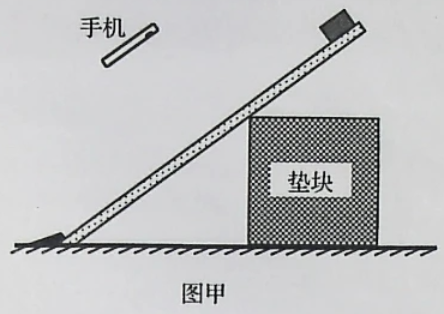
\includegraphics[]{img/image21.png}
\end{center}
(\romannumeral1)如图甲所示,选择合适高度的垫块,使木板的倾角为$53°$,在其上表面固定一与小物块下滑路径平行的刻度尺(图中未画出)。

(\romannumeral2)调整手机使其摄像头正对木板表面,开启视频录像功能。将小物块从木板顶端释放,用手机记录下小物块沿木板向下做加速直线运动的情况。然后通过录像的回放,选择小物块运动路径上合适的一点作为测量参考点,得到小物块相对于该点的运动距离L与运动时间t的数据。

(\romannumeral3)该同学选取部分实验数据,画出了$\frac{2L}{t}-t$图像,利用图像数据得到小物块下滑的加速度大小为$5.6m/s^2$。

(\romannumeral4)再次调节垫块,改变木板的倾角,重复实验.回答以下问题:

(1)当木板的倾角为$37°$时,所绘图像如图乙所示。由图像可得,物块过测量参考点时速度的大小为\key{0.32或0.33}$m/s;$选取图线上位于坐标纸网格交叉点上的A、B两点,利用A、B两点数据得到小物块下滑加速度的大小为\key{3.1}$m/s^2$。(结果均保留2位有效数字)

(2)根据上述数据,进一步分析得到当地的重力加速度大小为\key{9.4}$m/s^2$。(结果保留2位有效数字,$sin37^°=0.60$,$cos37°=0.80$)\begin{center}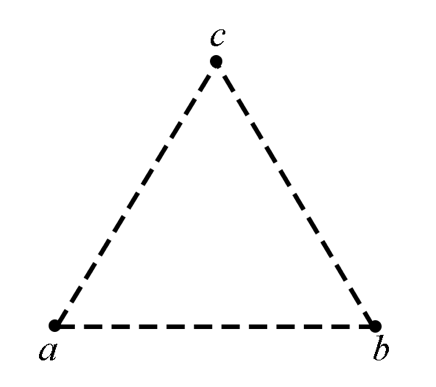
\includegraphics[]{img/image11.png}\end{center}



\question[6] (8分)实验方案对实验测量的精度有直接的影响,某学习小组对"测量电源的电动势和内阻"的实验方案进行了探究。实验室提供的器材有:

干电池一节(电动势约$1.5V$,内阻小于1Ω);

电压表V(量程3V,内阻约$3kΩ$);

电流表A(量程$0.6A$,内阻约1Ω);

滑动变阻器R(最大阻值为$20Ω$);

定值电阻$R_1$(阻值2Ω);

定值电阻$R_2$(阻值5Ω);

开关一个,导线若干。

(1)该小组按照图甲所示的电路进行实验,通过调节滑动变阻器阻值使电流表示数逐渐接近满偏,记录此过程中电压表和电流表的示数,利用实验数据在$U-I$坐标纸上描点,如图乙所示,结果发现电压表示数的变化范围比较小,出现该现象的主要原因是\key{B}。(单选,填正确答案标号)

A.电压表分流B.干电池内阻较小C.滑动变阻器最大阻值较小D.电流表内阻较小\begin{center}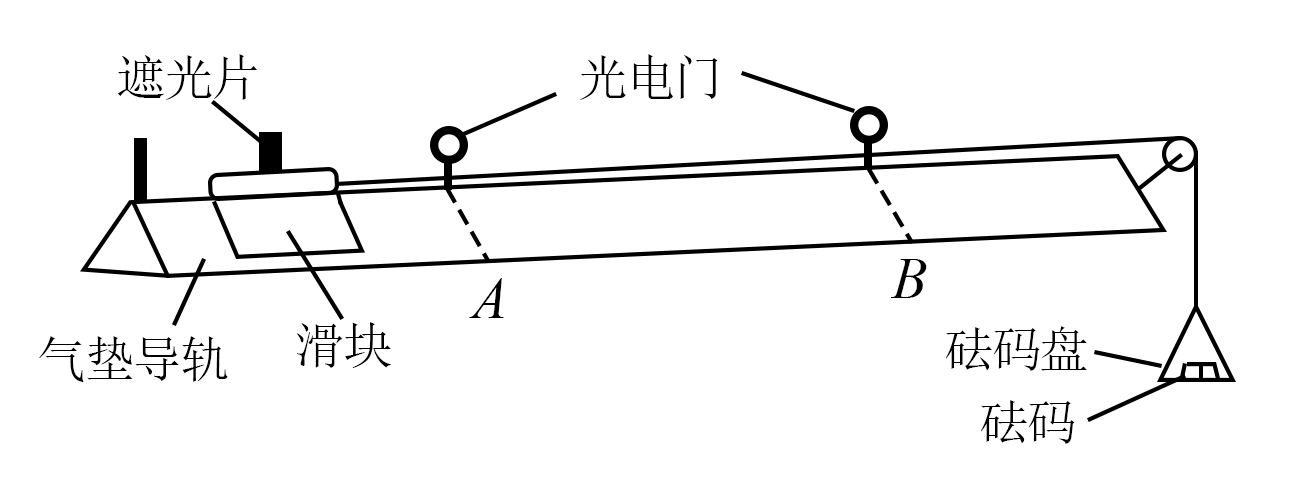
\includegraphics[]{img/image12.png}\end{center}

(2)针对电压表示数的变化范围比较小的问题,该小组利用实验室提供的器材改进了实验方案,重新测量得到的数据如下表所示。

\begin{table}[h]
    \begin{center}
        \begin{tabular}{|l|l|l|l|l|l|l|l|}
            \hline
            序号  & 1    & 2    & 3    & 4    & 5    & 6    & 7    \\ \hline
            I/A & 0.08 & 0.14 & 0.20 & 0.26 & 0.32 & 0.36 & 0.40 \\ \hline
            U/V & 1.35 & 1.20 & 1.05 & 0.88 & 0.73 & 0.71 & 0.52 \\ \hline
            \end{tabular}
    \end{center}
\end{table}
请根据实验数据,回答以下问题:

\ding{172}答题卡的坐标纸上已标出后3组数据对应的坐标点,请在答题卡的坐标纸上标出前4组数据对应的坐标点并画出$U-I$图像。

\ding{173}根据实验数据可知,所选的定值电阻为\key{$R_1$}(填$"R_1"$或$"R_2"$)。

\ding{174}用笔画线代替导线,请在答题卡上按照改进后的方案,将实物图连接成完整电路。

\newpage
\question[6] (7分)中医拔罐的物理原理是利用玻璃罐内外的气压差使罐吸附在人体穴位上,进而治疗某些疾病。常见拔罐有两种,如图所示,左侧为火罐,下端开口;右侧为抽气拔罐,下端开口,上端留有抽气阀门。使用火罐时,先加热罐中气体,然后迅速按到皮肤上,自然降温后火罐内部气压低于外部大气压,使火罐紧紧吸附在皮肤上。抽气拔罐是先把罐体按在皮肤上,再通过抽气降低罐内气体压强。某次使用火罐时,罐内气体初始压强与外部大气压相同,温度为$450K$,最终降到$300K$,因皮肤凸起,内部气体体积变为罐容积的$\frac{20}{21}$若换用抽气拔罐,抽气后罐内剩余气体体积变为抽气拔罐容积的$\frac{20}{21}$,罐内气压与火罐降温后的内部气压相同。罐内气体均可视为理想气体,忽略抽气过程中气体温度的变化。求应抽出气体的质量与抽气前罐内气体质量的比值。\begin{center}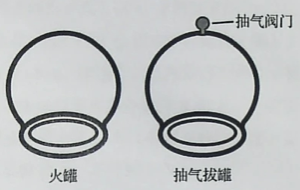
\includegraphics[]{img/image13.png}\end{center}
\begin{solution}{4cm}
    $\frac{\Delta m}{m}=\frac{1}{3}$
\end{solution}
\question[6] (9分)单板滑雪U型池比赛是冬奥会比赛项目,其场地可以简化为如图甲所示的模型:U形滑道由两个半径相同的四分之一圆柱面轨道和一个中央的平面直轨道连接而成,轨道倾角为$17.2°$。某次练习过程中,运动员以$v_A=10m/s$的速度从轨道边缘上的M点沿轨道的竖直切面$ABCD$滑出轨道,速度方向与轨道边缘线AD的夹角$α=72.8°$,腾空后沿轨道边缘的N点进入轨道。图乙为腾空过程左视图。该运动员可视为质点,不计空气阻力,取重力加速度的大小$g=10m/s^2$,$sin72.8°=0.96$,$cos72.8°=0.30.$求:

(1)运动员腾空过程中离开AD的距离的最大值d;

(2)M、N之间的距离L.\begin{center}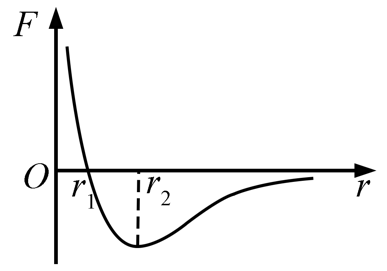
\includegraphics[]{img/image14.png}\end{center}
\begin{solution}{4cm}
    (1)d=4.8m

    (2)L=12m
\end{solution}
\newpage
\question[6] (14分)某型号质谱仪的工作原理如图甲所示。M、N为竖直放置的两金属板,两板间电压为U,Q板为记录板,分界面P将N、Q间区域分为宽度均为d的\uppercase\expandafter{\romannumeral1}、\uppercase\expandafter{\romannumeral2}两部分,M、N、P、Q所在平面相互平行,a、b为M、N上两正对的小孔。以a、b所在直线为z轴,向右为正方向,取z轴与Q板的交点O为坐标原点,以平行于Q板水平向里为x轴正方向,竖直向上为y轴正方向,建立空间直角坐标系$O_{xyz}$。区域\uppercase\expandafter{\romannumeral1}、\uppercase\expandafter{\romannumeral2}内分别充满沿x轴正方向的匀强磁场和匀强电场,磁感应强度大小、电场强度大小分别为B和E。一质量为m,电荷量为+q的粒子,从a孔飘入电场(初速度视为零),经b孔进入磁场,过P面上的c点(图中未画出)进入电场,最终打到记录板Q上.不计粒子重力。

(1)求粒子在磁场中做圆周运动的半径R以及c点到z轴的距离L;

(2)求粒子打到记录板上位置的x坐标;

(3)求粒子打到记录板上位置的y坐标(用R、d表示);

(4)如图乙所示,在记录板上得到三个点$s_1$、$s_2$、$s_3$,若这三个点是质子$_1^1H$、氚核$_1^3H$、氦核$_2^4He$的位置,请写出这三个点分别对应哪个粒子(不考虑粒子间的相互作用,不要求写出推导过程)。\begin{center}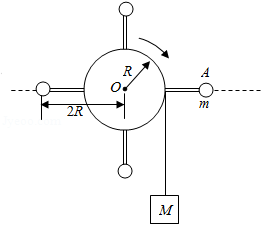
\includegraphics[]{img/image15.png}\end{center}
\begin{solution}{4cm}
    (1)$L=\frac{\sqrt{2mqU}}{qB}-\sqrt{\frac{2mU}{qB^2}-d^2}$

    (2)$x=\frac{md^2E}{4mU-2qd^2B^2}$

    (3)$y=R-\sqrt{R^2-d^2}+\frac{d^2}{\sqrt{R^2-d^2}}$

    (4)$s_1$、$s_2$、$s_3$分别对应氚核$_1^3H$、氦核$_2^4He$、质子$_1^1H$的位置
\end{solution}
\newpage
\question[6] (16分)如图所示,一倾角为θ的固定斜面的底端安装一弹性挡板,P、Q两物块的质量分别为m和4m,Q静止于斜面上A处。某时刻,P以沿斜面向上的速度$v_0$与Q发生弹性碰撞。Q与斜面间的动摩擦因数等于$tanθ$,设最大静摩擦力等于滑动摩擦力。P与斜面间无摩擦,与挡板之间的碰撞无动能损失。两物块均可以看作质点,斜面足够长,Q的速度减为零之前P不会与之发生碰撞。重力加速度大小为g。

(1)求P与Q第一次碰撞后瞬间各自的速度大小$v_{P1}$、$v_{Q1}﹔$

(2)求第n次碰撞使物块Q上升的高度$h_n;$

(3)求物块Ω从A点上升的总高度H;

(4)为保证在Q的速度减为零之前P不会与之发生碰撞,求A点与挡板之间的最小距离s。\begin{center}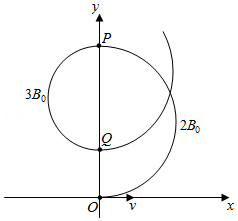
\includegraphics[]{img/image16.png}\end{center}
\begin{solution}{4cm}
    (1)$v_{P1}=\frac{3}{5}v_0$$v_{Q1}=\frac{2}{5}v_0$

    (2)$h_n=(\frac{7}{25})^{n-1}\cdot \frac{v_0^2}{25g}$(n=1,2,3……)

    (3)$H=\frac{v_0^2}{18g}$

    (4)$s=\frac{(8\sqrt{7}-13)v_0^2}{200g\sin\theta}$
\end{solution}